% benchmarks.tex — \input'd from experiments/experiments.tex
%
% Sources: experiments/data/benchmark.jsonl (self-contained timing dataset, generated by benchmark.rs)

\subsection{Benchmarks and Algorithm Selection}
\label{sec:benchmark}

We benchmark the HK2017 and billiard algorithms on random polytopes
($F = 5, \ldots, 12$) and Lagrangian products to establish practical
performance limits and guide algorithm selection. Table~\ref{tab:benchmark-stats}
shows timing statistics for HK2017 pruned on 83 random polytopes.

\begin{table}[h]
\centering
\begin{tabular}{rrrrrr}
\toprule
$F$ & $N$ & Median (ms) & Mean (ms) & Min (ms) & Max (ms) \\
\midrule
 5 & 10 &       0.5 &       0.5 &      0.4 &       0.6 \\
 6 & 10 &       3.1 &       3.5 &      2.1 &       6.5 \\
 7 & 10 &      16.9 &      17.3 &     13.3 &      25.2 \\
 8 & 15 &      64.6 &      71.0 &     44.0 &     127.2 \\
 9 & 15 &     353.2 &     415.4 &    196.2 &     969.6 \\
10 & 15 &   1{,}957 &   2{,}091 &    866.8 &   4{,}503 \\
11 &  5 &   8{,}099 &   7{,}825 &  3{,}375 &  11{,}890 \\
12 &  3 &  27{,}011 &  32{,}116 & 18{,}679 &  50{,}658 \\
\bottomrule
\end{tabular}
\caption{HK2017 pruned computation time for random 4-polytopes by facet count.}
\label{tab:benchmark-stats}
\end{table}

A log-linear regression on the median times yields
\[
  T_{\mathrm{pruned}}(F) \;=\; 2.3 \times 10^{-7} \cdot 4.8^F \quad\text{seconds}
  \qquad (R^2 = 0.998),
\]
with growth rate~${\sim}4\text{--}5\times$ per facet. Extrapolating to the
4D crosspolytope ($F = 16$), the model predicts ${\sim}19{,}600$~seconds
(5.4~hours) per capacity computation.

For $F \le 7$, we compare pruned vs unpruned on random polytopes
(Table~\ref{tab:pruned-vs-unpruned}). On Lagrangian products, the billiard
algorithm is consistently 2--3$\times$ faster than HK2017 pruned
(Table~\ref{tab:billiard-vs-hk2017}).

\begin{table}[h]
\centering
\begin{tabular}{rrrr}
\toprule
$F$ & Pruned (ms) & Unpruned (ms) & Speedup \\
\midrule
 5 &   0.5 &   0.4 & 0.8$\times$ \\
 6 &   3.1 &   3.5 & 0.9$\times$ \\
 7 &  16.9 &  26.6 & 1.6$\times$ \\
\bottomrule
\end{tabular}
\caption{Pruned vs unpruned timing for small random polytopes.}
\label{tab:pruned-vs-unpruned}
\end{table}

\begin{table}[h]
\centering
\begin{tabular}{rrrr}
\toprule
$F$ & Billiard (ms) & HK2017 pruned (ms) & Speedup \\
\midrule
 6 &     1.1 &     3.3 &   3.0$\times$ \\
 7 &     7.8 &    17.8 &   2.3$\times$ \\
 8 &    36.2 &    67.4 &   1.9$\times$ \\
 9 &   193.3 &   381.8 &   2.0$\times$ \\
10 &   925.6 & 1{,}941.7 &   2.1$\times$ \\
\bottomrule
\end{tabular}
\caption{Billiard vs HK2017 pruned on random Lagrangian products.}
\label{tab:billiard-vs-hk2017}
\end{table}

Based on these benchmarks, we adopt the following algorithm selection:

\begin{itemize}
  \item \textbf{Lagrangian products}: Use billiard (polynomial cost).
  \item \textbf{General polytopes}: Use HK2017 pruned. Practical limit:
    $F \le 12$ for routine datasets, $F \le 14$ for one-off computations.
  \item \textbf{Debug testing}: Use HK2017 unpruned on $F \le 7$ to exercise
    all code paths with internal assertions.
\end{itemize}

Figure~\ref{fig:benchmark-timing} shows all timing data with fitted exponential
models for each algorithm and polytope class.

\begin{figure}[h]
\centering
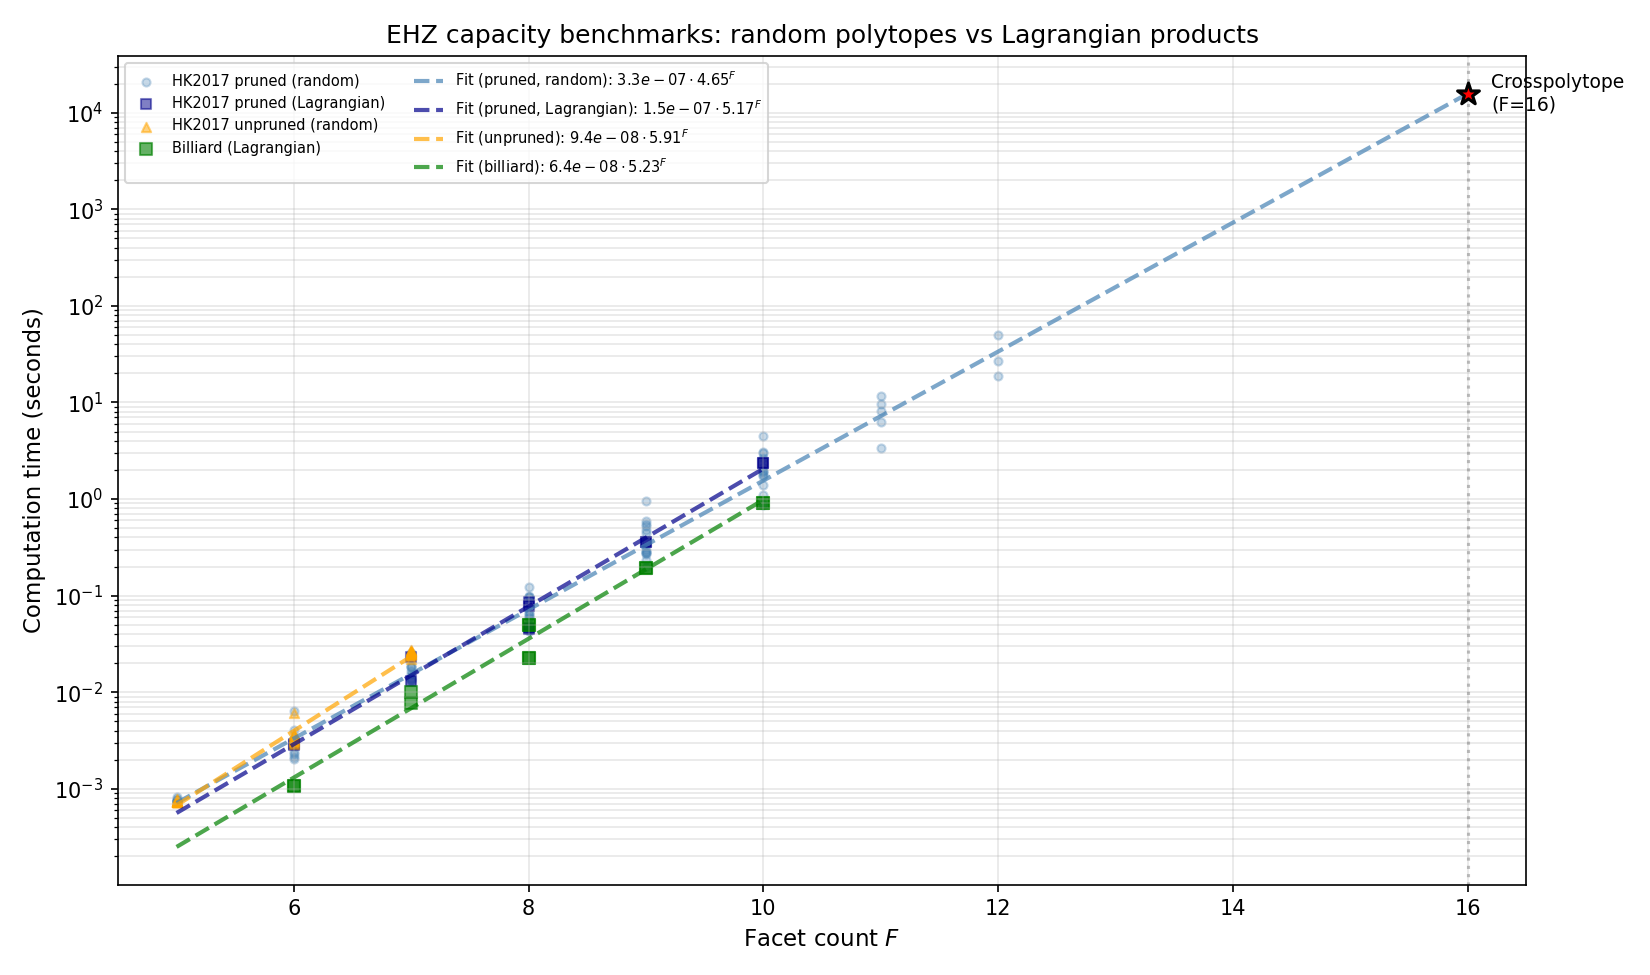
\includegraphics[width=0.95\textwidth]{../experiments/benchmark/benchmark_timing.png}
\caption{EHZ capacity benchmarks. Each algorithm and polytope class shows
  individual samples and a fitted exponential model. HK2017 pruned on random
  polytopes (fitted model extrapolated to crosspolytope, $F = 16$) shows the
  steepest growth. Billiard on Lagrangian products is consistently faster than
  HK2017 on the same polytope class.}
\label{fig:benchmark-timing}
\end{figure}
